\subsection{Polarizers and wave plates}
Date of carrying out experiment: 

\subsubsection{Brewster's angle}
\begin{enumerate}
    \item find Brester's angle \\
     only light polarized perpendicular to plane of incidence is reflected
     \\ $\Rightarrow$ polarization of reflected light is then linear
    \item take glass plate
    \item vary angle of incidence
    \item observations
    \item second glass plate (perpendicular planes of incidence)
\end{enumerate}

\subsubsection{Polarizers}
\begin{enumerate}
    \item calibrate (for that: find polarization axis)
    \item set reference for calibrating polarizers and PBS
\end{enumerate}

\subsubsection{Polarizing beam splitters}
\begin{enumerate}
    \item how is transmitted/reflected light polarized?
    \item calibrate
\end{enumerate}

\subsubsection{Wave-plates}
\begin{enumerate}
    \item find angle: half-waveplates rotate polarization by
    $\frac{\pi}{2}$ ($\alpha=45^\circ$)
    \item find angle: quarter-waveplates produce circular polarized
    light ($\alpha=45^\circ$)
    \item experiments from figure \ref{wave_plate_setup1} and
    \ref{wave_plate_setup2}
\end{enumerate}
\begin{figure}
\centering
\begin{subfigure}{.5\textwidth}
  \centering
  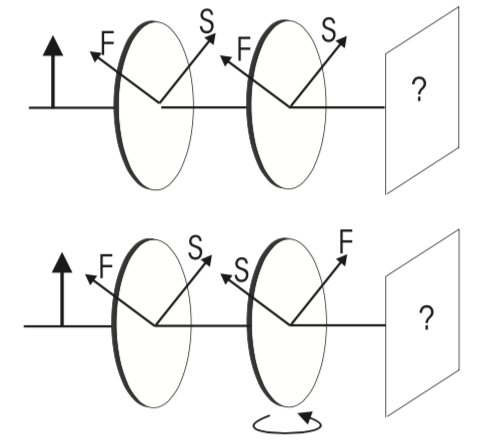
\includegraphics[width=.8\linewidth]{wave_plate_setup1}
  \caption{setup 1}
  \label{wave_plate_setup1}
\end{subfigure}%
\begin{subfigure}{.5\textwidth}
  \centering
  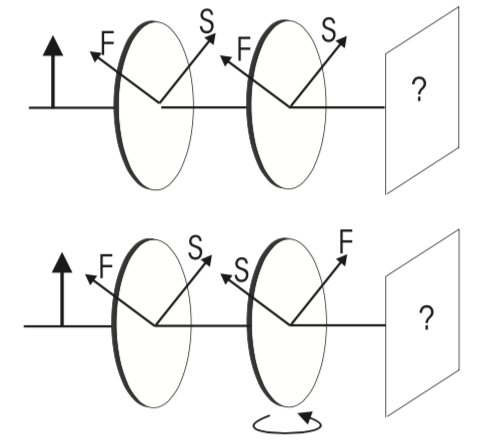
\includegraphics[width=.8\linewidth]{wave_plate_setup2}
  \caption{setup 2}
  \label{wave_plate_setup2}
\end{subfigure}
\caption{setups for wave-plate experiment}
\label{wave_plate_setup}
\end{figure}

\subsubsection{Mirror}
\begin{enumerate}
    \item measure polarization of reflected light
    \item send linear through two quarter-waveplates
    \item ...
\end{enumerate}

\subsubsection{Lamp light}
...

\newpage\ \newpage
\subsection{Electro-optical effect}
Date of carrying out experiment: \\
Material: LiNbO$_3$ (uniaxial crystal, $3m$-Symmetrie,
$n_1=n_2=n_o, n_3=n_e$)
\\ Pockels coefficients are very hard to measure, can be affected by crystal
impurities \\ \\

In the first part of this experiment, the change of the index of
refraction will be measured directly. In the second part, the
effect will be observed by measuring the polarization state of light 
before and after traversing the crystal.

\subsubsection{Phase shift due to electro-optical modulation}
\begin{enumerate}
    \item $\vec E$-field along optical axis
    \item laser beam is incident perpendicular to the field
    \item HV supply: output should be between $0$ V and $1.8$ kV
    \item measure amplification factor of HV amplifier
    \item evaluate measurements
\end{enumerate}

\subsubsection{Mach-Zehnder interferometer}
To quantify the extent by which the phase is shifted, we use a
Mach-Zehnder interferometer.
\begin{enumerate}
    \item why non-polarizing beam splitters
    \item direction of optical axes
    \item good overlap of arms
    \item setup measurement
    \item output intensity as function of applied voltage (for both axes)
    \item compare results
    \item just for fun: speaker
\end{enumerate}
\begin{figure}[h!]
    \center
    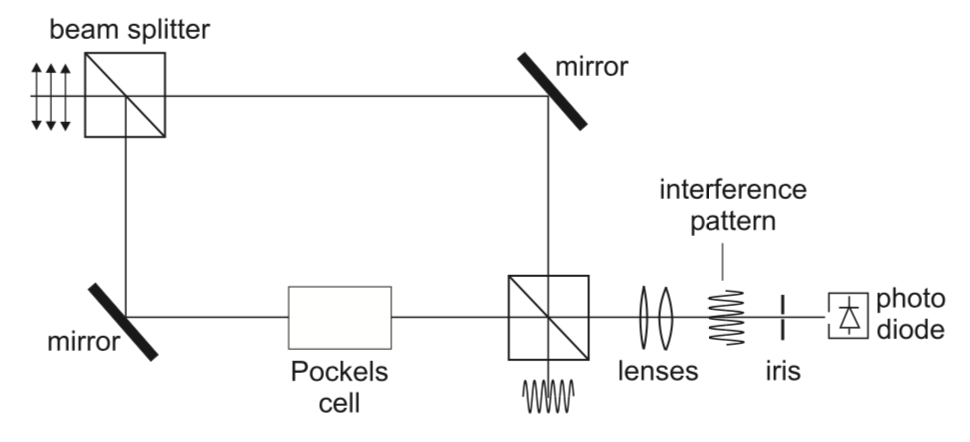
\includegraphics[width=.75\textwidth]{mach_zehnder_interferometer}
    \caption{setup of Mach-Zehnder interferometer}
    \label{mach_zehnder_interferometer}
\end{figure}

\subsubsection{Manipulation of polarization and intensity}
\begin{enumerate}
    \item why Pockels cell at $45^\circ$
    \item measure transmitted power as function of HV for $\pm45^\circ$
\end{enumerate}

\subsubsection{Linear amplitude modulation}
\begin{enumerate}
    \item ...
\end{enumerate}


\newpage\ \newpage
\subsection{Acousto-optical effect}
Date of carrying out experiment: 

\subsubsection{Experiments with a single AOM}
\begin{itemize}
    \item adjust AOM so that amplitude of diffraction pattern is
    approximately symmetric in both $\pm 1$ orders
    \item measure diffraction angles for order 1 and 2 for
    various frequencies
    \item measure power of order 1 maximum relative to power of undiffracted
    beam as a function of frequency (same steps as above)
    \item optimize power in order 1 max, ...
\end{itemize}

\subsubsection{Two perpendicular AOMs}
\begin{itemize}
    \item expectation of diffraction pattern? compare with results
    \item what happes when offset voltage(s) is/are changed?
\end{itemize}
